\documentclass{beamer}
\usepackage[english, russian]{babel}
\usepackage[utf8]{inputenc}
\usepackage[english,russian]{babel}
\setbeamertemplate{caption}[numbered]
\usepackage{comment}
\usepackage{amsmath,amsfonts,amssymb,mathtext,cite,enumerate,float,indentfirst,floatflt,setspace}
\usepackage{geometry}
\usepackage{multicol,subcaption,multirow}
\usepackage{graphicx,tocvsec2}
\usepackage[skip=2pt,font=tiny]{caption}
\usepackage{adjustbox,wrapfig,bm}
\usepackage{enumitem,layout}
\usepackage{csvsimple} % для импорта csv - таблиц

\setlist{nolistsep}
\usefonttheme[onlymath]{serif}
\hypersetup{unicode=true}
\usetheme{Boadilla}
\usecolortheme{rose}
\makeatletter
\newcommand\titlegraphicii[1]{\def\inserttitlegraphicii{#1}}
\titlegraphicii{}
\setbeamertemplate{title page}
{
  \vbox{}
   {\usebeamercolor[fg]{titlegraphic}\inserttitlegraphic\hfill\inserttitlegraphicii\par}
  \begin{centering}
    \begin{beamercolorbox}[sep=8pt,center]{institute}
      \usebeamerfont{institute}\insertinstitute
    \end{beamercolorbox}
    \begin{beamercolorbox}[sep=8pt,center]{title}
      \usebeamerfont{title}\inserttitle\par%
      \ifx\insertsubtitle\@empty%
      \else%
        \vskip0.25em%
        {\usebeamerfont{subtitle}\usebeamercolor[fg]{subtitle}\insertsubtitle\par}%
      \fi%     
    \end{beamercolorbox}%
    \vskip1em\par
    \begin{beamercolorbox}[sep=8pt,center]{author}
      \usebeamerfont{author}\insertauthor
    \end{beamercolorbox}
  \end{centering}
  %\vfill
}
\makeatother

\setbeamertemplate{footline}
{
  \leavevmode%
  \hbox{%
	\begin{beamercolorbox}[wd=.9\paperwidth,ht=2.25ex,dp=1ex,center]{author in head/foot}%
    \usebeamerfont{scriptsize}Применение различных вариантов метода декомпозиции
  \end{beamercolorbox}%
  \begin{beamercolorbox}[wd=.1\paperwidth,ht=2.25ex,dp=1ex,right]{title in head/foot}%
    \insertframenumber{} / \inserttotalframenumber\hspace*{1ex}
  \end{beamercolorbox}}%
  \vskip0pt%
}
	
\setbeamertemplate{navigation symbols}{}

\title{Применение различных вариантов  \\ метода декомпозиции \\ для численного решения \\ задач деформирования упругих тел}
\institute{МИНИСТЕРСТВО ОБРАЗОВАНИЯ И НАУКИ \\ РОССИЙСКОЙ ФЕДЕРАЦИИ \\ Федеральное агентство по образованию \\  МОСКОВСКИЙ ГОСУДАРСТВЕННЫЙ ТЕХНИЧЕСКИЙ УНИВЕРСИТЕТ ИМЕНИ Н.Э. БАУМАНА \\ Факультет "`Фундаментальные науки"' \\ Кафедра "`Прикладная математика"'}
\date{Москва, 2021 г.}

\begin{document}

\begin{frame}[plain]
\maketitle
\tiny
\begin{tabular}[t]{@{\hspace{150pt}}l@{\hspace{10pt}}l@{}}
Исполнитель: & Матвеев Михаил \\
Научный руководитель: & канд. физ.-мат. наук  \\
& Родин Александр Сергеевич
\end{tabular}
\centering
\bigskip 

\insertdate
\end{frame}
\begin{frame}
\small
\begin{block}{Цель}
Исследование сходимости итерационного цикла при решении задач деформирования упругих тел различными методами декомпозиции области
\end{block}
\begin{block}{Задачи}
\begin{itemize}
\item[-]применение МКЭ для решения задач теории упругости;
\medskip
\item[-]реализация различных методов Шварца;
\medskip
\item[-]анализ применения мультипликативного, аддитивного и двухуровневого аддитивного методов Шварца при решении ряда задач упругого деформирования тела;
\end{itemize}
\end{block}
\end{frame}

\begin{frame}{Постановка задачи механики твёрдого деформируемого тела}
\small
Уравнения равновесия в деформируемом теле, занимающем область $G$ с границей $\partial \, G$:
\begin{equation*}
L \mathbf{u} = - \triangledown \bm{\sigma(u)} = \mathbf{f(x)}, \ x \in G
\end{equation*}
с кинематическими и силовыми граничными условиями
\begin{equation*}
\bm{u(x)} = u_0, \ x \in \partial \, G_D,
\end{equation*}
\begin{equation*}
\bm{\sigma}\mathbf{(u) \cdot n} = \mathbf{p(x)}, \ x \in \partial \, G_N,
\end{equation*}
где $\partial \, G_D$ - участок границы области $G$, на котором заданы кинематические условия, $\partial \, G_N$ - участок границы области $G$, на котором заданы силовые условия.

\end{frame}

\begin{frame}{Основные положения для метода Шварца}
\begin{multicols}{2}

Рассмотрим произвольную область $G$, разделённую на конечное число подобластей $G = \bigcup_{i=1}^{M} G_i$ с внутренними границами $\partial G_1, \ldots, \partial G_M$. 
\vspace{1cm}

Данные подобласти пересекаются, необходимо ввести дополнительные обозначения граничных значений:
\begin{equation*}
\begin{array}{l}
\partial G_{N, i} = \partial G_N \cap \partial G_i \\
\partial G_{D, i} = \partial G_D \cap \partial G_i \\
\partial \tilde{G_i} = G \setminus ((G_i \setminus \partial G_i) \cap \partial G_{N, i}) 
\end{array}
\end{equation*}

\columnbreak
\begin{figure}[h]
\center{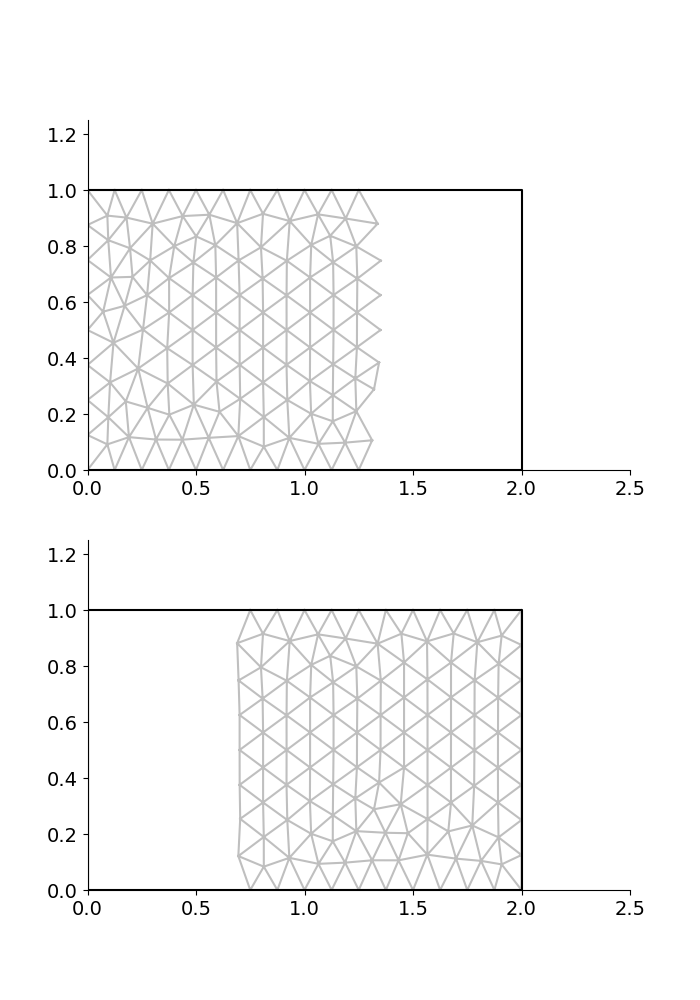
\includegraphics[scale=0.3]{../results/rectangle/3_fixes/core/area_decomposition.png}}
\caption{Схема декомпозиции расчётной области}
\end{figure}
\end{multicols}
\end{frame}

\begin{frame}{Мультипликативный и аддитивный методы Шварца}
\footnotesize
\begin{multicols}{2}
Основные формулы мультипликативного метода Шварца:
\begin{equation*}
\begin{array}{ll}
L \; (u^{n+\frac{i}{M}}) = f(x), & x \in G_i \\
\sigma(u^{n+\frac{i}{M}}) \cdot n = p(x), & x \in \partial G_{N, i} \\
u^{n+\frac{i}{M}}(x) = 0, & x \in \partial G_{D, i} \\ 
u^{n+\frac{i}{M}}(x) = u^{n+\frac{(i - 1)}{M}}(x), & x \in \partial \tilde{G_i}
\end{array}
\end{equation*}

Мультипликативный метод Шварца последователен, решение на каждой итерации зависит от решения на предыдущей подобласти. 

\columnbreak

Основные формулы аддитивного метода Шварца:
\begin{equation*}
\begin{array}{rl}
L (u^{n+\frac{i}{M}}) = f(x), & x \in G_i \\
\sigma(u^{n+\frac{i}{M}}) \cdot n = p(x), & x \in \partial G_{N, i} \\
u^{n+\frac{i}{M}}(x) = 0, & x \in \partial G_{D, i} \\ 
u^{n+1}(x) = u^{n}(x), & x \in \partial \tilde{G_i}
\end{array}
\end{equation*}

В конце каждой итерации решение вычисляется по формуле:
\begin{equation*}
u^{n+1} = u^{n} + \alpha \sum_{i=1}^{M} (u_i^{n+1} - u^{n}),
\end{equation*}
где коэффициент $\alpha$ - итерационный параметр, от которого зависит скорость сходимости итерационного процесса. 
\end{multicols}
\end{frame}

\begin{frame}{Двухуровневый аддитивный метод Шварца}
\footnotesize
\begin{multicols}{2}
Для улучшения сходимости метода Шварца используются двухуровневые методы, заключающиеся в наличии помимо основной сетки грубой сетки.

Для двухуровневого аддитивного метода Шварца решение на каждой итерации ищется по формуле
\begin{equation*}
u^{n+1} = u^n + \alpha\sum_{i=1}^{M} {(u_i^{n+1} - u^n)} + \alpha \Delta \hat{u}_0^{n+1},
\end{equation*}
где $\Delta \hat{u}_0^{n+1}$ - решение задачи, полученное на грубой сетке и пересчитанное на узлы основной сетки путём интерполяции.

Решение в узлах грубой сетки ищется по формуле

\begin{equation*}
\mathbf{K_c} \Delta u_0^{n+1} = \mathbf{R_c}^{n+1}
\end{equation*}

\columnbreak

\begin{figure}[h]
\center{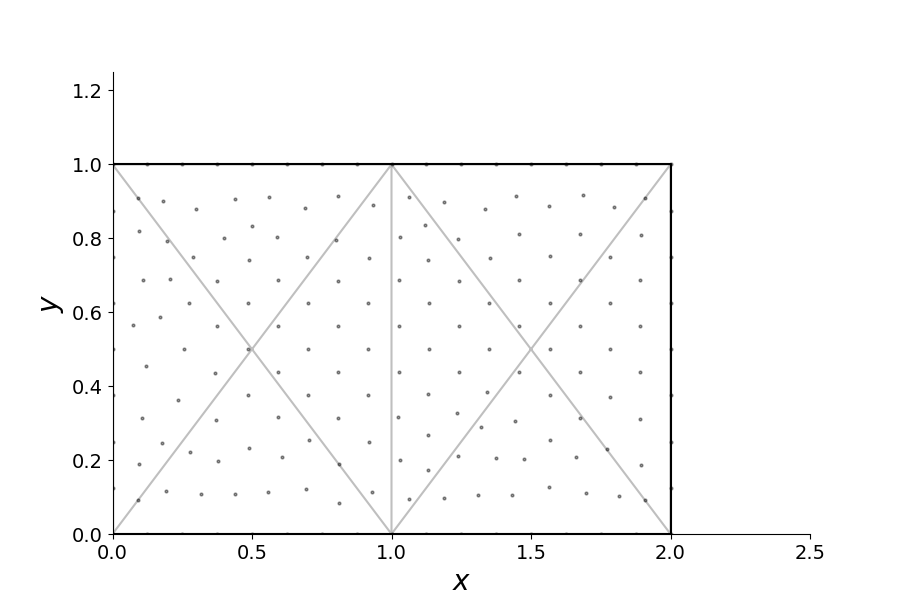
\includegraphics[scale=0.25]{../results/rectangle/3_fixes/core/area_coarse_rectangle.png}}
\caption{Схема расчётной области с прямоугольной областью в качестве грубой области}
\end{figure}

Вектор правой части для грубой сетки вычисляется по формуле

\begin{equation*}
\mathbf{R_c^{n+1}} = \mathbf{A} \mathbf{r^n},
\end{equation*}
где $\mathbf{r^n}$ - вектор невязки в узлах базовой сетки, $\mathbf{A}$ - интерполяционная матрица.

\begin{equation*}
\Delta \hat{u}_0^{n+1} = \mathbf{F} \Delta u_0^{n+1}
\end{equation*}

\end{multicols}
\end{frame}

\begin{frame}{Первая тестовая задача}
\framesubtitle{Основные сведения и таблицы}
\footnotesize
\begin{multicols}{2}
Расчётная область - прямоугольник, закреплённый с левой стороны по оси OX и с нижней стороны по оси OY. Внешнее давление $p$ = 50 МПа, ширина тела $a = 2$ см, высота тела $b = 1$ см.
\vspace{-1cm}
\begin{figure}[h]
\center{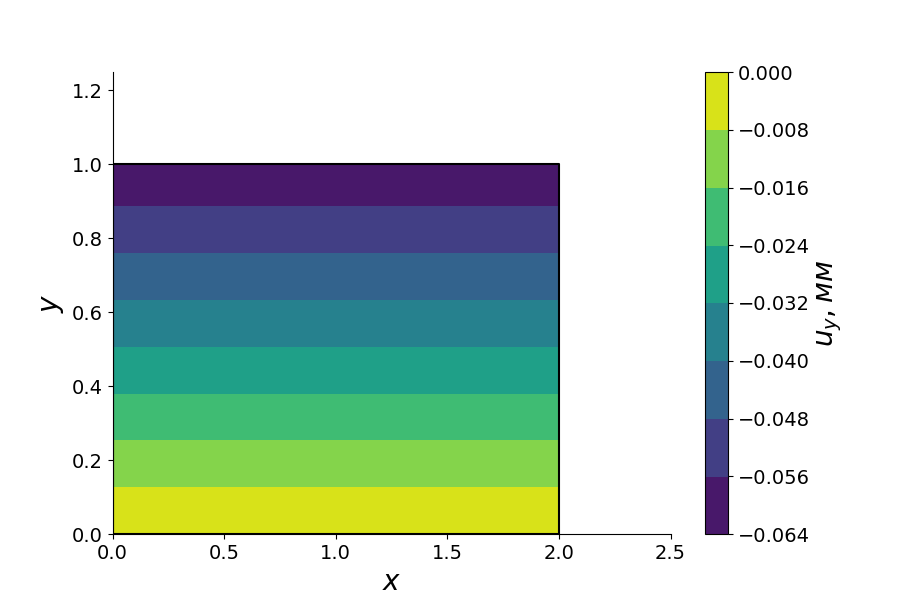
\includegraphics[scale=0.25]{../results/rectangle/2_fixes/core/displacement_distribution.png}}
\caption{Распределение перемещений во всей расчётной области}
\end{figure}

\columnbreak

\begin{table}[h]	
\begin{center}
\begin{adjustbox}{max width=0.5\textwidth}
\begin{tabular}{|@{}c@{}|@{\hspace{0.1em}}c@{}|@{\hspace{0.3em}}c@{\hspace{0.3em}}|@{\hspace{0.3em}}c@{\hspace{0.3em}}|@{\hspace{0.3em}}c@{\hspace{0.3em}}|@{\hspace{0.3em}}c@{\hspace{0.3em}}|}
\hline
МДО & M & h = 0.05 & h = 0.025 & h = 0.0125 & h = 0.00625 \\ \hline
\multirow{3}{*}{Мульт}
& 2 & 23 & 23 & 23 & 22 \\ \cline{2-6}
& 4 & 102 & 100 & 99 & 99 \\ \cline{2-6}
& 8 & 401 & 386 & 385 & 383 \\ \hline
\multicolumn{6}{|c|}{}\\ 
\hline
\multirow{3}{*}{Адд}
& 2 & 80 & 79 & 79 & 78 \\ \cline{2-6}
& 4 & 346 & 338 & 336 & 334 \\ \cline{2-6}
& 8 & 1303 & 1254 & 1251 & 1250 \\ \hline
\multicolumn{6}{|c|}{}\\ 
\hline
\multirow{3}{*}{2Адд}
& 2 & 15 & 15 & 14 & 15 \\ \cline{2-6}
& 4 & 14 & 14 & 16 & 15 \\ \cline{2-6}
& 8 & 1 & 16 & 17 & 17 \\ \hline
\end{tabular}
\end{adjustbox}
\end{center}
\caption{Таблица количества итераций в зависимости от количества подобластей и шага мелкой сетки}
\end{table}

\vspace{-1cm}

\begin{table}[h]	
\begin{center}
\begin{adjustbox}{max width=0.5\textwidth}
\begin{tabular}{|p{2cm}|@{\hspace{0.1em}}c@{}|@{\hspace{0.3em}}c@{\hspace{0.3em}}|@{\hspace{0.3em}}c@{\hspace{0.3em}}|@{\hspace{0.3em}}c@{\hspace{0.3em}}|}
\hline
Количество подобл-тей & H = 1 & H = 0.5 & H = 0.25 & H = 0.125 \\ \hline
2 & 17 & 15 & 14 & 14 \\
\hline
4 & 29 & 19 & 16 & 16 \\ 
\hline
8 & 42 & 26 & 17 & 17 \\ 
\hline
\end{tabular}
\end{adjustbox}
\end{center}
\caption{Таблица количества итераций в зависимости от количества подобластей и шага грубой сетки}
\end{table}

\end{multicols}
\end{frame}

\begin{frame}{Вторая тестовая задача}
\framesubtitle{Основные сведения и таблицы}
\footnotesize
\begin{multicols}{2}
Расчётная область - сектор поперечного сечения толстостенной трубы, нагруженной внешним давлением. Внутренний радиус $r_a = 1$ см, внешний радиус $r_b = 2$ см, внешнее давление $p = 5$ МПа.
\begin{figure}[h]
\center{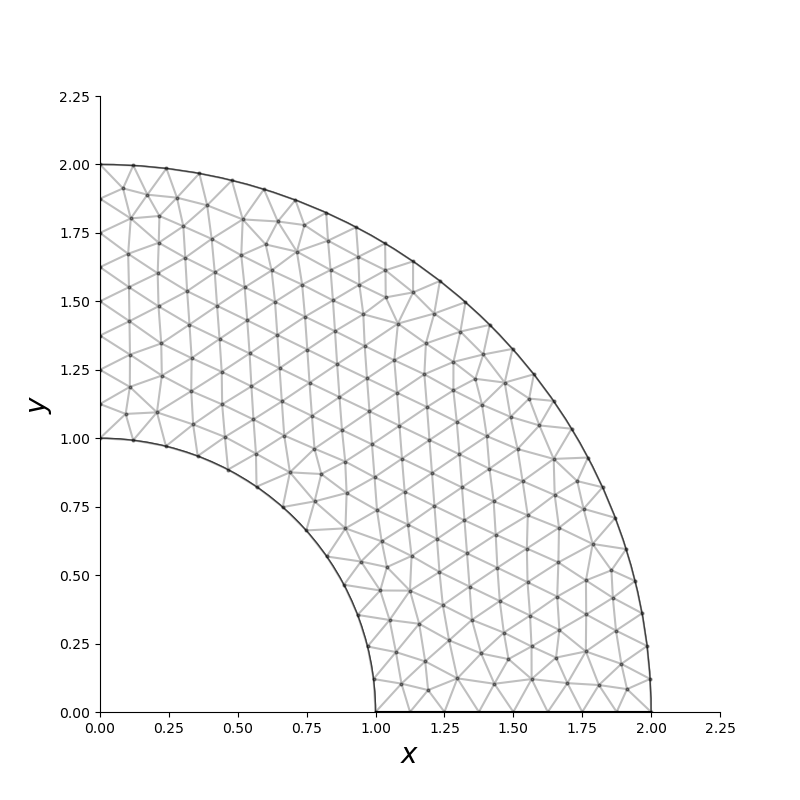
\includegraphics[scale=0.25]{../results/thick_walled_cylinder/pressure_only/core/area_diagram.png}}
\end{figure}

\columnbreak

\begin{table}[h]	
\begin{center}
\begin{adjustbox}{max width=0.5\textwidth}
\begin{tabular}{|@{}c@{}|@{\hspace{0.1em}}c@{}|@{\hspace{0.3em}}c@{\hspace{0.3em}}|@{\hspace{0.3em}}c@{\hspace{0.3em}}|@{\hspace{0.3em}}c@{\hspace{0.3em}}|@{\hspace{0.3em}}c@{\hspace{0.3em}}|}
\hline
МДО & M & h = 0.05 & h = 0.025 & h = 0.0125 & h = 0.00625 \\ \hline
\multirow{3}{*}{Мульт}
& 2 & 44 & 44 & 44 & 43 \\ \cline{2-6}
& 4 & 178 & 169 & 169 & 168 \\ \cline{2-6}
& 8 & 528 & 497 & 494 & 488 \\ \hline
\multicolumn{6}{|c|}{}\\ 
\hline
\multirow{3}{*}{Адд}
& 2 & 68 & 38 & 40 & 42 \\ \cline{2-6}
& 4 & 128 & 170 & 110 & 120 \\ \cline{2-6}
& 8 & 463 & 408 & 393 & 398 \\ \hline
\multicolumn{6}{|c|}{}\\ 
\hline
\multirow{3}{*}{2Адд}
& 2 & 15 & 15 & 14 & 15 \\ \cline{2-6}
& 4 & 14 & 14 & 16 & 15 \\ \cline{2-6}
& 8 & 16 & 16 & 17 & 17 \\ \hline
\end{tabular}
\end{adjustbox}
\end{center}
\caption{Таблица количества итераций в зависимости от количества подобластей и шага мелкой сетки}
\end{table}

\vspace{-1cm}

\begin{table}[h]	
\begin{center}
\begin{adjustbox}{max width=0.5\textwidth}
\begin{tabular}{|p{2cm}|@{\hspace{0.1em}}c@{}|@{\hspace{0.3em}}c@{\hspace{0.3em}}|@{\hspace{0.3em}}c@{\hspace{0.3em}}|}
\hline
Количество подобл-тей & H = 0.5 & H = 0.25 & H = 0.125 \\ \hline
2 & 17 & 16 & 15 \\
\hline
4 & 21 & 19 & 15 \\ 
\hline
8 & 23 & 19 & 17 \\ 
\hline
\end{tabular}
\end{adjustbox}
\end{center}
\caption{Таблица количества итераций в зависимости от количества подобластей и шага грубой сетки}
\end{table}

\end{multicols}
\end{frame}

\begin{frame}{Вторая тестовая задача}
\framesubtitle{Аналитические решения}
\footnotesize
Для толстостенного цилиндра известно аналитическое решение:
\begin{equation*}
u=\frac{\left(1-2\nu\right)\left(1+\nu\right)}{E} \frac{(p_a \cdot r_a^2 - p_b \cdot r_b^2)}{(r_b^2 - r_a^2)}r+\frac{1+\nu}{E}\frac{(r_a r_b)^2}{r}\frac{(p_a - p_b)}{(r_b^2 - r_a^2)},
\end{equation*}
\begin{equation*}
\sigma_{rr}=\frac{(p_a \cdot r_a^2 - p_b \cdot r_b^2)}{b^2-a^2}-\frac{a^2 b^2}{r^2}\frac{(p_a - p_b)}{b^2 -a^2},
\end{equation*}
\begin{equation*}
\sigma_{\varphi\varphi}=\frac{(p_a \cdot r_a^2 - p_b \cdot r_b^2)}{b^2-a^2}+\frac{a^2 b^2}{r^2}\frac{(p_a - p_b)}{b^2 -a^2}.
\end{equation*}

\begin{table}
\centering
\begin{tabular}{|c|c|c|c|}
\hline
Шаг сетки & $u_r$ & $\sigma_r$ & $\sigma_\varphi$\\
\hline
0.05 & 1.39$\times 10^{-4}$ & 2.93$\times 10^{-2}$ & 1.13$\times 10^{-2}$ \\
\hline
0.025 & 3.50$\times 10^{-5}$ & 1.42$\times 10^{-2}$ & 5.60$\times 10^{-3}$ \\
\hline
0.0125 & 8.72$\times 10^{-6}$ & 7.04$\times 10^{-3}$ & 2.84$\times 10^{-3}$ \\
\hline
\end{tabular}
\caption{Ошибки численного решения}
\end{table}

\begin{table}
\centering
\begin{tabular}{|c|c|c|c|}
\hline
Шаг сетки & $u_r$ & $\sigma_r$ & $\sigma_\varphi$\\
\hline
0.05 & 1 & 1 & 1 \\
\hline
0.05 & 4.1 & 2.5 & 2.02 \\
\hline
0.05 & 16.21 & 4.46 & 4.28 \\
\hline
\end{tabular}
\caption{Отношение ошибок численного решения}
\end{table}

\end{frame}

\begin{frame}{Вторая тестовая задача}
\framesubtitle{Дополнительные графики}
\begin{multicols}{2}
\begin{figure}[h]
\center{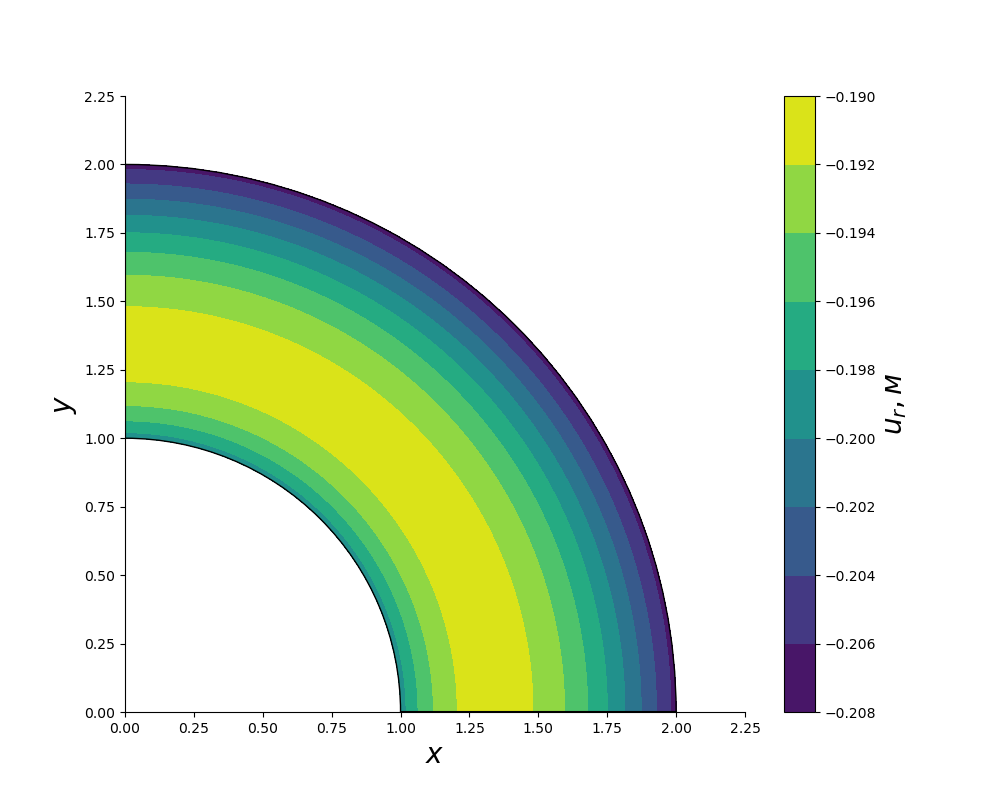
\includegraphics[scale=0.23]{../results/thick_walled_cylinder/pressure_only/core/displacement_distribution.png}}
\caption{Распределение узловых перемещений во всей области}
\end{figure}
\columnbreak
\begin{figure}[h]
\center{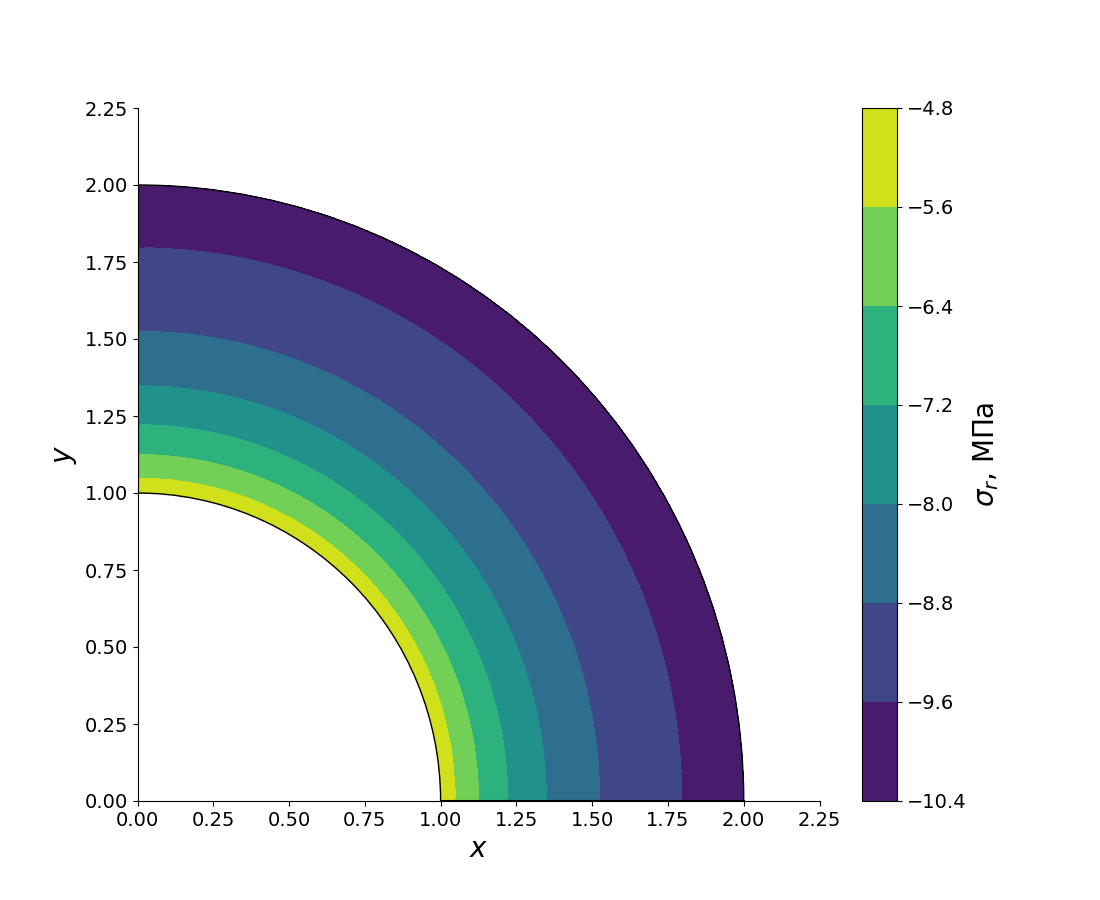
\includegraphics[scale=0.23]{../results/thick_walled_cylinder/pressure_only/core/pressure_distribution_r.png}}
\caption{Распределение узловых радиальных напряжений во всей области}
\end{figure}
\end{multicols}
\end{frame}

\begin{frame}{Третья тестовая задача}
\framesubtitle{Основные сведения и таблицы}
\footnotesize
\begin{multicols}{2}
Расчётная область - сектор поперечного сечения модели подшипника, нагруженной внешним давлением. Внутренний радиус $r_a = 1$ см, внешний радиус $r_b = 2$ см, внешнее давление $p = 5$ МПа.
\begin{figure}[h]
\center{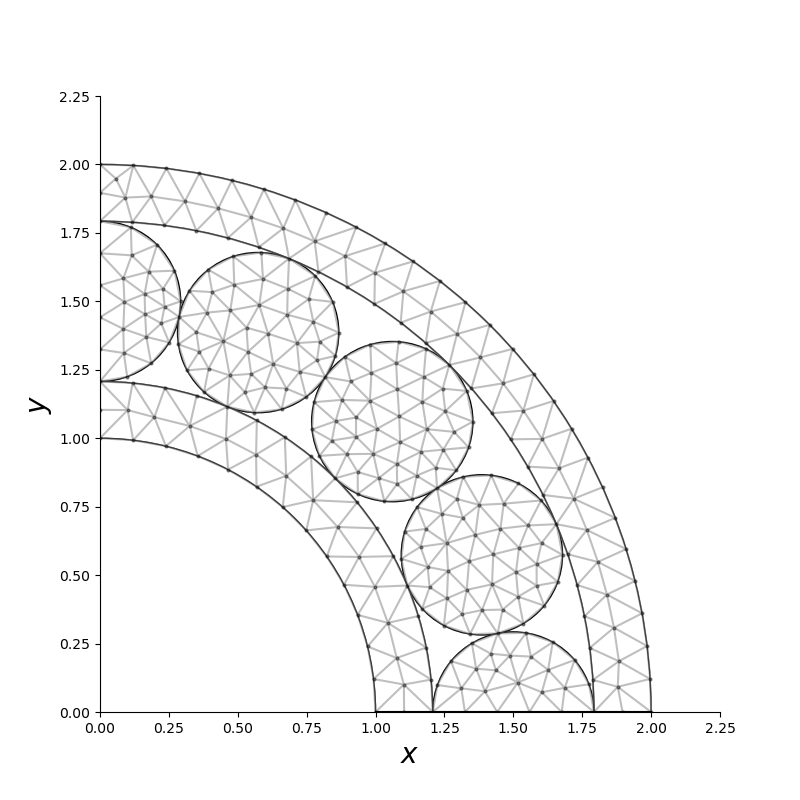
\includegraphics[scale=0.25]{../results/bearing/pressure_only/core/area_diagram.png}}
\end{figure}

\columnbreak

\begin{table}[h]	
\begin{center}
\begin{adjustbox}{max width=0.5\textwidth}
\begin{tabular}{|@{}c@{}|@{\hspace{0.1em}}c@{}|@{\hspace{0.3em}}c@{\hspace{0.3em}}|@{\hspace{0.3em}}c@{\hspace{0.3em}}|@{\hspace{0.3em}}c@{\hspace{0.3em}}|@{\hspace{0.3em}}c@{\hspace{0.3em}}|}
\hline
МДО & M & h = 0.05 & h = 0.025 & h = 0.0125 & h = 0.00625 \\ \hline
\multirow{3}{*}{Мульт}
& 2 & 42 & 44 & 45 & 48 \\ \cline{2-6}
& 4 & 220 & 231 & 245 & 261 \\ \cline{2-6}
& 8 & 409 & 509 & 550 & 592 \\ \hline
\multicolumn{6}{|c|}{}\\ 
\hline
\multirow{3}{*}{Адд}
& 2 & 52 & 36 & 49 & 50 \\ \cline{2-6}
& 4 & 194 & 184 & 183 & 182 \\ \cline{2-6}
& 8 & 647 & 566 & 546 & 550 \\ \hline
\multicolumn{6}{|c|}{}\\ 
\hline
\multirow{3}{*}{2Адд}
& 2 & 17 & 18 & 18 & 19 \\ \cline{2-6}
& 4 & 24 & 26 & 24 & 24 \\ \cline{2-6}
& 8 & 29 & 30 & 28 & 28 \\ \hline
\end{tabular}
\end{adjustbox}
\end{center}
\caption{Таблица количества итераций в зависимости от количества подобластей и шага мелкой сетки}
\end{table}

\vspace{-1cm}

\begin{table}[h]	
\begin{center}
\begin{adjustbox}{max width=0.5\textwidth}
\begin{tabular}{|p{2cm}|@{\hspace{0.3em}}c@{\hspace{0.3em}}|@{\hspace{0.3em}}c@{\hspace{0.3em}}|@{\hspace{0.3em}}c@{\hspace{0.3em}}|}
\hline
Количество подобл-тей & H = 0.5 & H = 0.25 & H = 0.125 \\ \hline
2 & 23 & 20 & 18 \\
\hline
4 & 39 & 31 & 24 \\ 
\hline
8 & 52 & 42 & 28 \\ 
\hline
\end{tabular}
\end{adjustbox}
\end{center}
\caption{Таблица количества итераций в зависимости от количества подобластей и шага грубой сетки}
\end{table}

\end{multicols}
\end{frame}

\begin{frame}{Третья тестовая задача}
\framesubtitle{Дополнительные графики}
\footnotesize
\begin{multicols}{2}
\begin{figure}[h]
\center{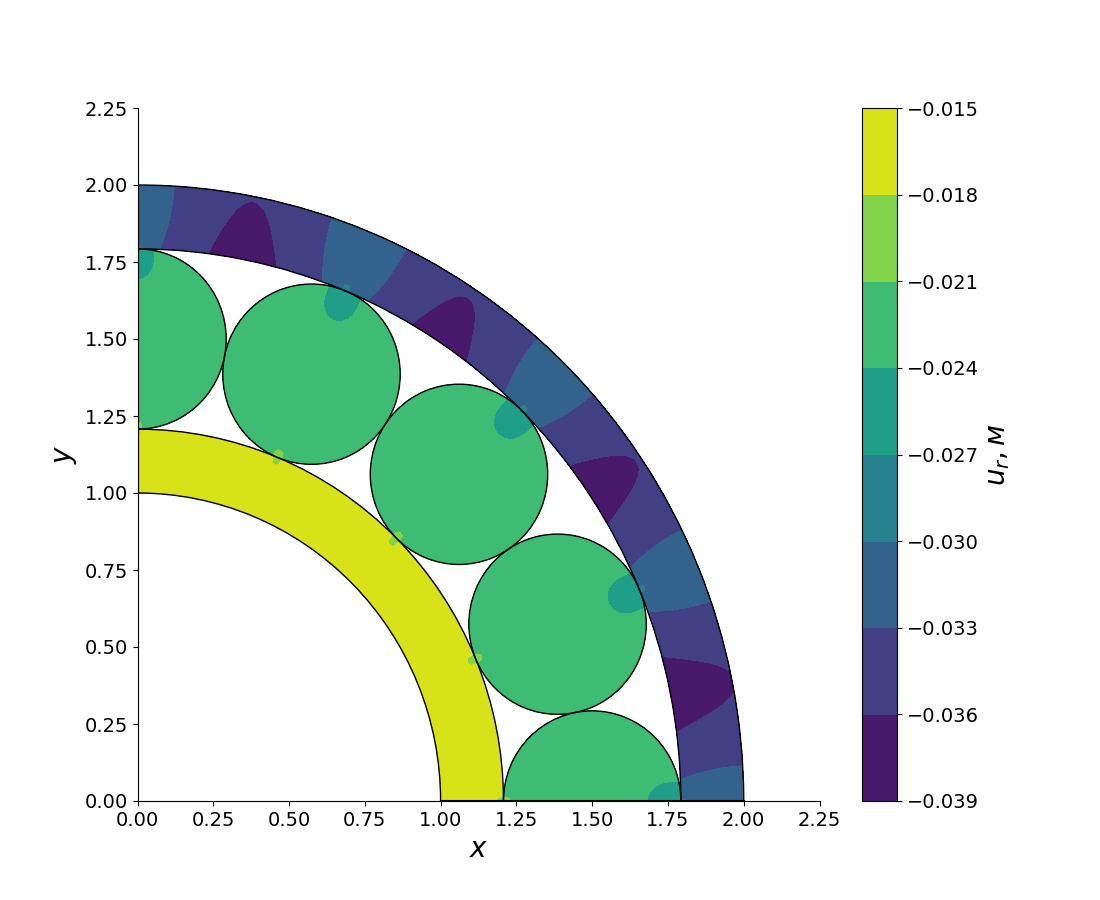
\includegraphics[scale=0.23]{../results/bearing/pressure_only/core/displacement_distribution.png}}
\caption{Распределение узловых перемещений во всей области}
\end{figure}
\columnbreak
\begin{figure}[h]
\center{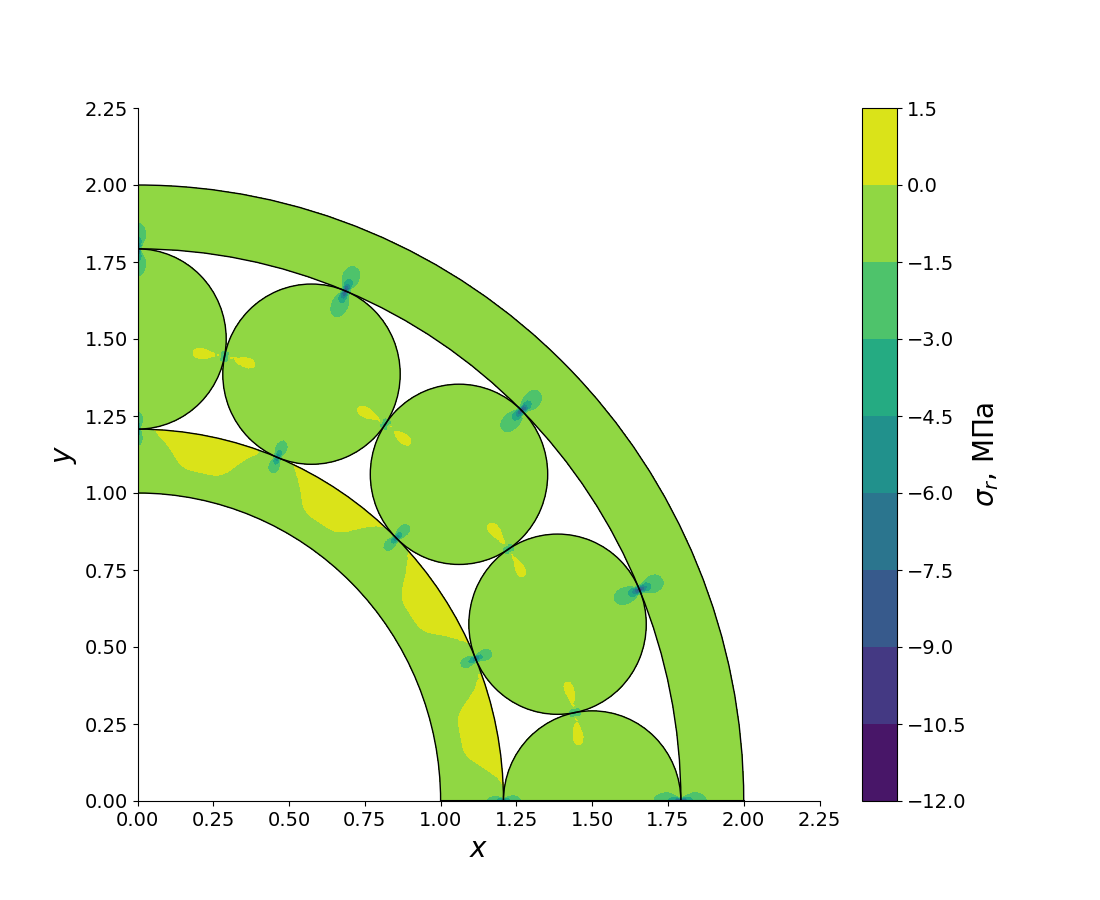
\includegraphics[scale=0.23]{../results/bearing/pressure_only/core/pressure_distribution_r.png}}
\caption{Распределение узловых радиальных напряжений во всей области}
\end{figure}
\end{multicols}
\end{frame}

\begin{frame}{Третья тестовая задача}
\framesubtitle{Анализ временных затрат}
\begin{table}
\begin{adjustbox}{max width=0.9\textwidth}
\begin{tabular}{|c|c|p{2.8cm}|p{2.8cm}|p{2.8cm}|p{2.8cm}|}
\hline
Размерность задачи & Базовый метод & Двухуровневый аддитивный метод (M = 2) & Двухуровневый аддитивный метод (M = 4) & Двухуровневый аддитивный метод (M = 8) & Двухуровневый аддитивный метод (M = 16) \\
\hline
9142 & 1.54 & 6.01 & 7.47 & 9.4 & 14.86 \\
\hline
33272 & 6.84 & 25.36 & 30.98 & 38.01 & 51.98 \\
\hline
127674 & 49.28 & 153.99 & 149.7 & 179.16 & 211.52 \\
\hline
497796 & 423.57 & 1319.15 & 1284.39 & 919.38 & 931.23 \\
\hline
\end{tabular}
\end{adjustbox}
\caption{Таблица временных затрат}
\end{table}

\begin{table}
\begin{adjustbox}{max width=\textwidth}
\begin{tabular}{|p{2cm}|p{2.3cm}|l|p{1.5cm}|p{2.8cm}|p{2.8cm}|p{2.8cm}|p{2.8cm}|}
\hline
Размерность задачи & Отношение размерностей & Теория & Базовый метод & Двухуровневый аддитивный метод (M = 2) & Двухуровневый аддитивный метод (M = 4) & Двухуровневый аддитивный метод (M = 8) & Двухуровневый аддитивный метод (M = 16) \\
\hline
9142 & 1 & 1 & 1 & 1 & 1 & 1 & 1 \\
\hline
33272 & 3.63 & 6.91 & 4.44 & 4.21 & 4.14 & 4.04 & 3.49 \\
\hline
127674 & 13.96 & 52.15 & 32 & 25.62 & 20.04 & 19.05 & 14.23 \\
\hline
497796 & 54.45 & 401.78 & 275.05 & 219.5 & 171.93 & 97.81 & 62.6 \\
\hline
\end{tabular}
\end{adjustbox}
\caption{Таблица отношений временных затрат}
\end{table}
\end{frame}

\begin{frame}

\begin{figure}[h]
\center{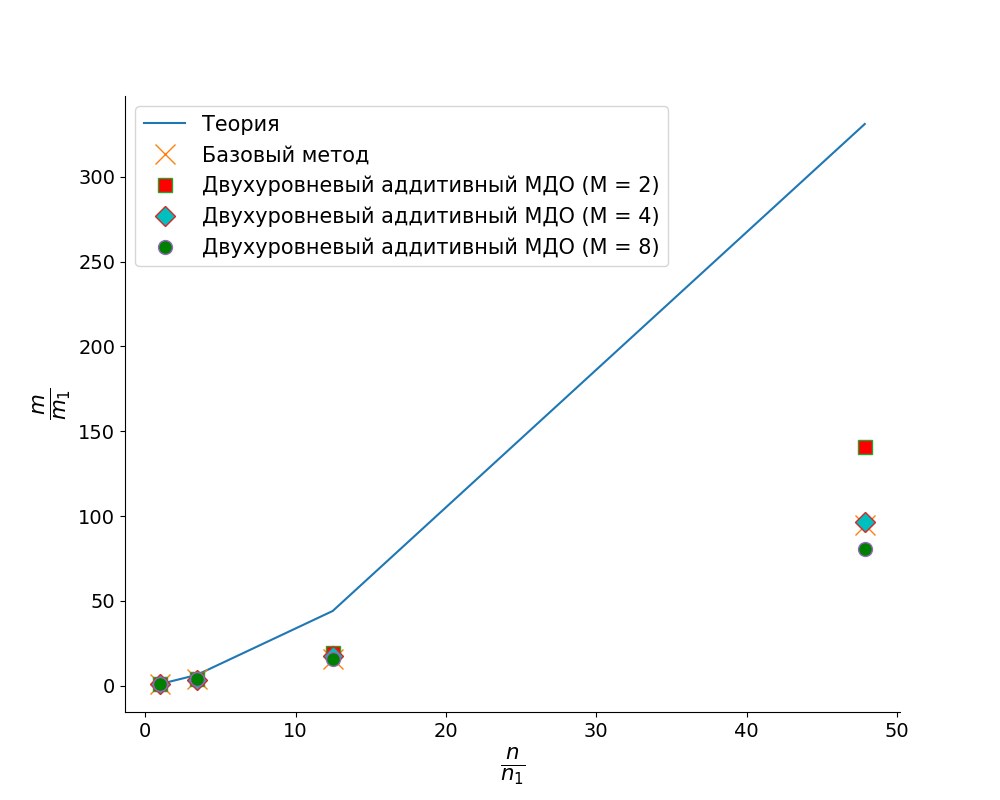
\includegraphics[scale=0.4]{../results/bearing/pressure_only/core/time_cg.png}}
\caption{График отношений временных затрат}
\end{figure}

\end{frame}

\begin{frame}{Заключение}
\small
\begin{itemize}
\item[-]Применён МКЭ для решения упругих задач
\medskip
\item[-]реализованы мультипликативный, аддитивный и двухуровневый аддитивный методы Шварца для численного решения задачи упругости;
\medskip
\item[-]проведены серии расчётов для ряда тестовых задач;
\medskip
\item[-]исследована зависимость сходимости путём сравнения количества итераций для мультипликативного, аддитивного и двухуровневого аддитивного методов Шварца от шага сетки и количества вводимых подобластей;
\medskip
\item[-]изучены скорости роста итераций и временных затрат при решении задачи методом сопряженных градиентов.
\end{itemize}
\end{frame}

\begin{frame}{Спасибо за внимание!}

\end{frame}
\end{document}
